\documentclass[pidr]{tnreport}
%\documentclass[confidential,pidr]{tnreport} % If you are writing confidential report

\usepackage{multirow}
\usepackage[]{algorithm2e}
\usepackage{float}

\def\reportTitle{Comparateur d'algorithmes de plus court chemin} % Titre du mémoire
\def\reportLongTitle{Benchmarking d'algorithmes de plus court chemins sur grilles générées par graine} % Titre plus long du mémoire

\def\reportAuthor{Vincent \textsc{Albert}\\ Nicolas \textsc{Bédrine}}
\def\reportAuthorEmail{\email{vincent.albert@telecomnancy.eu}\\ \email{nicolas.bedrine@telecomnancy.eu}} % Courriel de l'élève

\def\reportSupervisor{M.~Olivier Buffet} % Prénom Nom de l'encadrant industriel

\def\reportCompany{Loria} % Nom de l'entreprise d'accueil
\def\reportCompanyAddress{615, Rue du Jardin botanique}  % Adresse de l'entreprise
\def\reportCompanyCity{54506, Vandœuvre-lès-Nancy} % Adresse (cont.) de l'entreprise
\def\reportCompanyPhone{03 83 59 20 00} % Téléphone de l'entreprise
\def\reportCompanyLogoPath{figures/loria.jpg} % Logo de l'entreprise -- comment this definition to remove company logo

\def\place{Villers-lès-Nancy} % Ville pour la signature pour l'engagement anti-plagiat
\def\date{\today} % Date pour la signature de l'engagement anti-plagiat

\def\reportProjectCustomer{Projet réalisé pour l'équipe Maia du laboratoire Loria}

\titlespacing{\chapter}{0pt}{*-5}{*5}

\begin{document}
  
\maketitle
\pagenumbering{roman}

\insertAntiPlagiarismAgreement{\textsc{Albert}, Vincent}{1205033068}
\insertAntiPlagiarismAgreement{\textsc{Bédrine}, Nicolas}{0905020230}

\clearpage
\makesecondtitle

\section*{Remerciements}
\addcontentsline{toc}{chapter}{Remerciements}

{\em
Nous tenons à remercier toutes les personnes nous ayant accompagnés durant la réalisation de ce projet, et en particulier M.~\textsc{Buffet} pour nous avoir encadré et pour nous avoir prodigué ses précieux conseils. \\
Nous remercions aussi M.~Jean-François \textsc{Scheid} qui a supervisé l'organisation des PIDRs et de Mme~Isabelle \textsc{Chenet}, secrétaire des PIDRs. \\
Enfin, nous remercions toute l'équipe pédagogique et administrative de TELECOM Nancy pour nous fournir un cadre d'études adéquat à la réalisation de ce projet. \\
}

\clearpage

\section*{Avant-propos}
\addcontentsline{toc}{chapter}{Avant-propos}
\paragraph{}
Ce rapport est le résultat d'un projet de découverte de la recherche de quatre mois effectué dans le cadre du sujet fourni par M.~Olivier \textsc{Buffet}, chercheur au Loria.

\paragraph{}
Le projet a été réalisé pour l'équipe Maia (MAchines Intelligentes Autonomes), groupe de recherches centré sur les comportements décisionnels intelligents. Ses principaux champs de recherches sont les systèmes multi-agents et complexes ainsi que les systèmes décisionnels incertains.

\paragraph{}
N'ayant que peu d'expérience dans le domaine de l'Intelligence Artificielle mais étant très intéressés par cette dernière, nous avons choisi ce sujet afin d'en approfondir nos connaissances. 

\paragraph{}
Notre méconnaissance de la plupart des algorithmes de plus courts chemin nous a poussé à nous demander quelles en sont les principales différences. Notre étude portant sur l'implémentation des algorithmes ainsi que de leurs comparaison au travers de batteries de tests était donc l'occasion d'en apprendre plus sur leur fonctionnement.

\clearpage

\renewcommand{\baselinestretch}{0.5}\normalsize
\tableofcontents
\renewcommand{\baselinestretch}{1.0}\normalsize
\clearpage

\pagenumbering{arabic}
\setcounter{page}{1}

\chapter{Introduction}

	\section{État actuel du domaine de recherches et légitimité du sujet}

\paragraph{}
Les algorithmes de plus court chemin appartiennent à la théorie des graphes et constituent un vaste champ de recherches de l'Intelligence Artificielle. Il existe de nombreux algorithmes qui ont été développés depuis les débuts de la Recherche Opérationnelle au début des années 1940, les plus connus étant Dijkstra et A*.

\paragraph{}
Cependant, bien que ces algorithmes soient connus et maîtrisés, il est difficile de déterminer \textit{a priori} leur comportement sur différents types d'environnements, et donc de savoir lequel sera le plus efficace. \newline

	\section{Présentation du fonctionnement global et de l'utilisation du logiciel}

\paragraph{}
Le projet se propose donc de permettre de réaliser des séquences de tests de différents algorithmes sélectionnés par l'utilisateur sur des environnements différents générés par graine.

		\subsection{Fonctionnement du projet}
		
			\subsection{Les environnements}

\paragraph{}
Les environnements correspondent aux graphes sur lesquels les algorithmes sont appliqués. Il existe deux types d'algorithmes : les algorithmes générés sous forme de grilles à N dimensions avec N > 1 (hypercubes\footnote{Un hypercube est une version généralisée du carré à N dimensions}) et des environnements générés de manière totalement aléatoires.
			
			\subsection{Les algorithmes}
				
\paragraph{}
Plusieurs algorithmes de calcul de plus court chemin ont été choisis parmi différent algorithmes proposées afin de tester leur efficacité sur différents types d'environnements de différentes tailles. Nous avons choisis des algorithmes ayant des démarches et des volontés d'optimisations très différentes. Si certains vont trouver un compromis entre mémoire et temps de calcul, d'autres vont rechercher l'économie en mémoire. Certains de ces algorithmes ont d'ailleurs une recherche objective. Le but a été de rassemblé des algorithmes au profil différent pour comparer leur comportement. Leur point de départ et d'arrivée sont définis aléatoirement. Les algorithmes parcourent le graphe en explorant ses nœuds par accès directs.
		
							
		\subsection{Lancer le projet}

\paragraph{}
Afin de répondre à tout type de besoins, le jar exécutable du logiciel prend en paramètre plusieurs options permettant différents modes d'expérimentation.

			\subsubsection{En vue graphique}

\paragraph{}
En lançant le logiciel avec la commande : \emph{java -jar AlgoComparator.jar --view}, celui-ci se lance en mode graphique. Cependant cette option a été implémentée au début du développement, avant que nous nous rendions compte qu'elle ne nous était pas utile. Elle a donc été délaissée et n'est plus fonctionnelle.

\begin{figure}[!ht]
    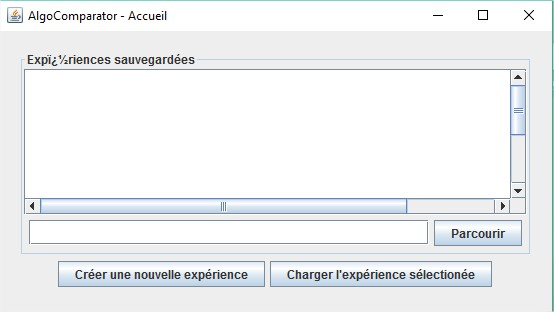
\includegraphics[width=0.5\textwidth]{./figures/ac_accueil.jpg}
    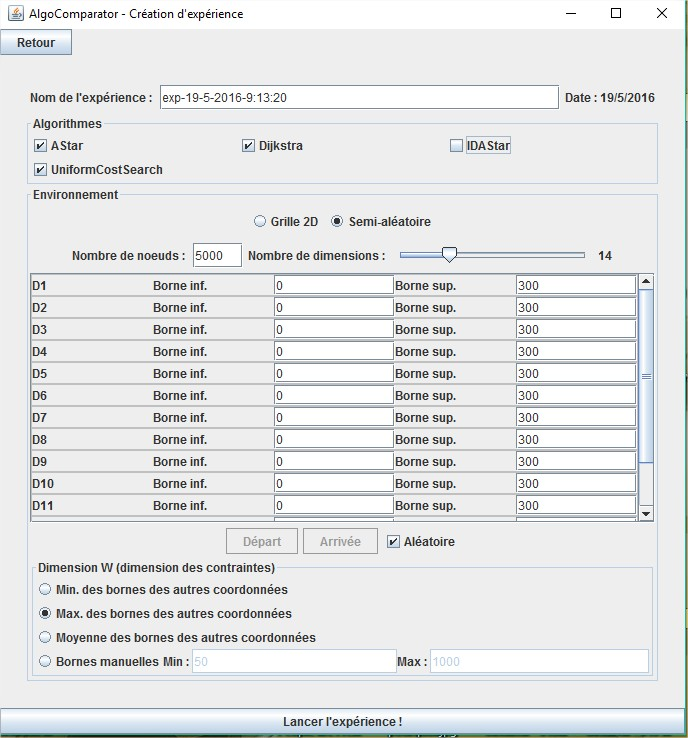
\includegraphics[width=0.5\textwidth]{./figures/ac_exp.jpg}
    \caption{Test graphique de création d'une grille}
\end{figure}

			\subsubsection{En console avec dialogue utilisateur}

\paragraph{}
En lançant le logiciel avec la commande : \emph{java -jar AlgoComparator.jar --console}, celui-ci se lance en mode console et initie un dialogue avec l'utilisateur. Il lui permettra de créer un environnement, de sauvegarder la graine, de lancer une expérience et d'enregistrer les résultats dans un fichier de logs.

			\subsubsection{En console en mode de benchmarking}
			
%\paragraph{}
En lançant le logiciel avec la commande : \emph{java -jar AlgoComparator.jar --bench}, celui-ci se lance en mode benchmarking. Il va charger la configuration dans le fichier bench.conf afin de déterminer la taille et le nombre de dimensions des environnements à générer. Un seul dialogue se lance avec l'utilisateur en début d'exécution pour lui demander les algorithmes qu'il veut lancer. Tous les résultats sont stockés dans le fichier "logs.txt". \newline
\emph{Note: l'option --bench all permet de lancer un benchmarking sur tous les algorithmes existants et supprime la séquence de dialogue.}
\cite{AIMA}
			
			\subsubsection{Tester la génération d'environnements}

\paragraph{}
Etant donné que nous avons rencontré des difficultés lors de la génération des environnements durant une certaine période du développement, nous avons aussi ajouté une option permettant de lancer un benchmarking sur la création d'environnements de 10 à plusieurs millions de points. Cette option est accessible avec la commande \emph{java -jar AlgoComparator.jar --test consenv}. \newline
Il est aussi possible d'avoir le test de l'affichage graphique d'un environnement en remplaçant l'option \textsc{consenv} par l'option \textsc{graphenv}. Ceci peut-être pratique pour vérifier que la création des liens entre les points se fait correctement.

\begin{figure}[H]
	\centering
    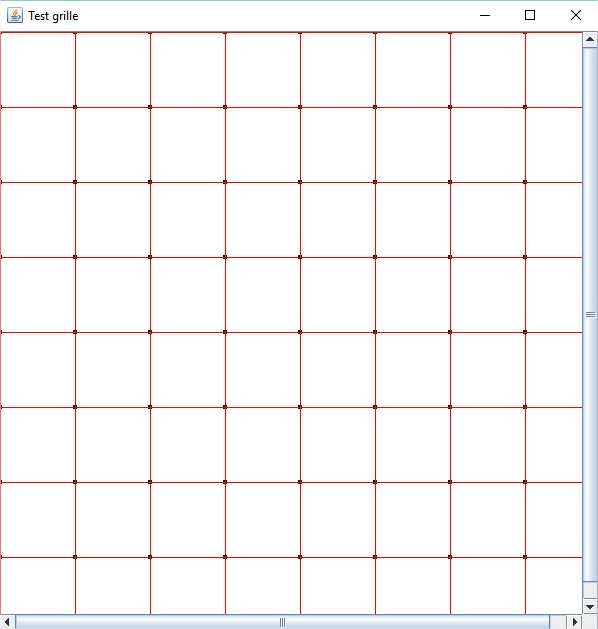
\includegraphics[width=0.6\textwidth]{./figures/ac_grille.jpg}
    \caption{Test graphique de création d'une grille}
\end{figure}

\clearpage

\chapter{Matériel et Méthode}

\paragraph{}
Nous allons maintenant voir les procédés mis en place pour le bon déroulement du projet et les outils développés afin de parvenir au résultat final.

	\section{Déroulement du projet}

		\subsection{Son organisation}

\paragraph{}
Afin d'avoir le meilleur suivi possible de l'avancement du projet, une réunion a été organisée avec l'encadrant toutes les deux semaines durant toute le période de développement du projet. En dehors de ces réunions, nous nous rencontrions afin de développer le projet en commun. Le reste du temps, nous avons programmé à distance grâce à l'utilitaire git. Le dépôt est accessible depuis le lien suivant : \url{https://github.com/PIDRGroup/AlgorithmComparator}.

		\subsection{Les technologies utilisées}

\paragraph{}
Le projet a été réalisé en Java sous Eclipse. \newline
Afin de travailler au mieux en équipe et de pouvoir gérer les versions de notre projet, nous avons utilisé le gestionnaire de version git. \newline
		
	\section{Outils développés pour tester les algorithmes}
	
\paragraph{}
Afin de tester les algorithmes, nous avons codé des outils nous permettant de tester l'efficacité des algorithmes que nous allons présenter ci-dessous.

		\subsection{Les environnements}

\paragraph{}
Le premier et plus important de ces outils est le générateur d'environnements permettant de tester un algorithme sous plusieurs configurations possibles.

			\subsubsection{Présentation générale de la conception des environnements : listes d'adjacence}
			
\paragraph{}
Tous les environnements sont conçus de la même façon. Ce sont des ensembles de places (représentées par N coordonnées pour N dimensions) reliées entre elles par des liens pondérés. Afin de représenter ces liens, nous possédons une liste d'adjacence associant à chacun des points la liste de ses successeurs. Chacune des dimensions possède une borne supérieure et inférieure.
	
			\subsubsection{Les environnements aléatoires}

\paragraph{}
Au début du projet, nous voulions générer aléatoirement des graphes orientés. Cependant nos premiers échecs furent infructueux ; nos graphes n'étaient en effet jamais suffisamment connexes pour qu'une solution existe. Nous avons alors recherché un moyen de générer un environnement aléatoire, orienté et fortement connexes, mais ils semblerait que cela soit encore du domaine de la recherche. Ceci n'étant pas l'axe principal de notre projet, nous avons décidé d'abandonner ce type de graphe afin de nous concentrer sur lagénération de grilles.
			
			\subsubsection{Les grilles et hypercubes}
		
\paragraph{}
Le principal type d'environnement utilisé sont donc les grilles à N dimensions. A partir des bornes données par l'utilisateur et le nombre de places appartenant à chaque dimension du graphe, les places sont générées de manière régulière sur chaque dimension. En parallèle de la création des points, chacun d'entre eux est relié à son voisin. On sait que dans un hypercube, tous les points ont pour voisins directs les points ayant exactement un coordonnées différente. A partir de là il est facile de générer le lien entre la place courante et tous les points qui ont été précédemment générés. \newline
Les liens sont pondérés pseudo-aléatoirement à partir d'un RNG alimenté par une graine spécifique (dans notre cas, le timestamp).
		
			\subsubsection{Génération d'environnement par graine : l'objet Seed}

\paragraph{}
Afin d'enregistrer facilement les données relatives à un graphe sans enregistrer la totalité des points (ce qui pourrait être une  perte considérable de place dans le cas d'un environnement à plusieurs millions de points), nous enregistrons toutes les données nécessaires à la génération d'un environnement dans un fichier texte, ce qui nous permettra par la suite de recréer exactement le même environnement sans sauvegarder tous les points. 

\paragraph{}
Les données enregistrées sont la graine (le timestamp lors de la première création de l'environnement), le nombre de points pour chacune des dimensions (nous sommes dans le cas des grilles et hypercubes) ainsi que la borne min et la borne inf des points (toutes les bornes sont considérées comme identiques, les hypercubes sont donc réguliers).

\paragraph{}
L'objet Seed de notre programme permet, à partir d'un fichier texte formaté, de reproduire à l'identique le graphe d'une environnement.

			\subsubsection{Les dimensions non-uniformes}
\paragraph{}
Il a été décidé d'implémenter un système de dimension non uniforme. La valeur d'un chemin pouvant varier selon sa position sur la carte, quand bien même sa distance euclidienne n'aurait pas changer. Cela permet de simuler la présence sur une carte d'un relief difficile. 

			\subsubsection{Les refactorisations du modèle des environnements}

\paragraph{}
Étant donné qu'au début nous désirions créer des environnements aléatoires, l'ensemble du code de nos Environnements se basait sur les positions des places dans le graphe. Or de cette manière, des parcours supplémentaires étaient obligatoires afin de rechercher des places par leurs coordonnées, ce qui ralentissait considérablement notre code. 
\paragraph{}
Cependant une fois les graphes aléatoires abandonnés, nous nous sommes rendus qu'il était bien plus facile et rapide de générer les graphes en grille à partir de leurs indices. Nous avons donc développé une seconde version plus efficace (étant donné que le nombre de dimensions et de points par dimension est connu à l'avance).
\paragraph{}
Cependant en effectuant des recherches, nous avons vu le principe de génération d'hypercubes de dimension N récursivement par fusion d'hypercubes de dimension N-1. Nous avons donc décidé d'adapter ce principe à nos grilles en N dimensions et à M points.

Voici les images exposant ce principe et dont nous nous sommes inspirés : 

\begin{figure}[H]
    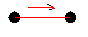
\includegraphics[width=0.15\textwidth]{./figures/Hypercube-dim1.PNG}
    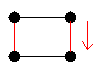
\includegraphics[width=0.15\textwidth]{./figures/Hypercube-dim2.PNG}
    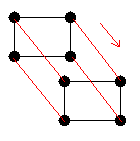
\includegraphics[width=0.2\textwidth]{./figures/Hypercube-dim3.PNG}
    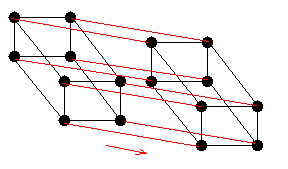
\includegraphics[width=0.4\textwidth]{./figures/Hypercube-dim4.PNG}
    \caption{Génération d'un hypercube en 4 dimensions}
\end{figure}

\paragraph{}
Nous avons donc refactorisé le code des Environnements afin d'appliquer cette modification, et la différence fut flagrante. Alors qu'il était impossible de générer un environnement d'un million de points dans la première version (même après plusieurs heures), le nouvel algorithme était capable de le faire en moins d'une dizaine de secondes. \newline
Voici l'algorithme que nous avons implémenté : 

\begin{algorithm}[H]
 \KwData{M : tableau qui associe à chaque dimension i son nombre de points, N : nombre de dimensions du graphe, borne\_inf : borne inférieure de toutes les dimensions, borne\_sup : borne supérieure de toutes les dimensions, i : compteur correspondant à la dimension courante, j : compteur correspondant au nombre de points de la dimension courante, graph : graph actuel que l'on fait évoluer}
 \KwResult{Hypercube de N dimensions à M[i] points chacune}

  graph = new Point(nb\_dim = N, coordonnées = \{borne\_min, ...\}) //On crée le point extremum  \newline
 i = 0 \newline
 \While{i < N}{
 //On calcule la distance entre les points de la dimension courante \newline
 	distance = calculerDist(M[i], borne\_inf, borne\_sup)  \newline
 	//On duplique le graphe le nombre de fois qu'il faut \newline
 	\For{j=0; j<M[i]; j++}{
 		tmp = dupliquer(graph) \newline
 		//On décale les coordonnées de la copie de la distance qui existe entre les points \newline
 		glisser\_coordonnées(tmp, distance) \newline
 		copies\_graph.push(tmp) \newline
 	}
 	graph = fusion(graph, copies\_graph) //On fusionne toutes les copies ensembles
 }
 \caption{Algorithme de génération d'une grille à N dimensions}
\end{algorithm}

\paragraph{}
Le tableau \ref{label_env} compare les différentes versions de l'algorithme de création de grilles à N dimensions.

\begin{table}[h]
\begin{center}
   \begin{tabular}{| l || r | r | r || r | r | r || r | r | r || r | r | r || r | r | r || r | r | r || r | r | r |}
     \hline
      \textbf{Version} & \multicolumn{3}{c||}{\textbf{10\up{2}}} & \multicolumn{3}{c||}{\textbf{10\up{4}}} & \multicolumn{3}{c||}{\textbf{10\up{6}}} & \multicolumn{3}{c||}{\textbf{10\up{7}}} \\
     \hline
     \cline{2-5}
    & \textbf{2D} & \textbf{3D} & \textbf{4D} & \textbf{2D} & \textbf{3D} & \textbf{4D} & \textbf{2D} & \textbf{3D} & \textbf{4D} & \textbf{2D} & \textbf{3D} & \textbf{4D}\\ \hline
     1\up{ère} version & 5 & - & - & ~10\up{7} & ~10\up{8} & ~10\up{8} & \multicolumn{3}{c||}{+$\infty$}  & \multicolumn{3}{c||}{+$\infty$}   \\ \hline
     2\up{ème} version & 2 & - & - & 34 & 36 & 41 & 16 864 & 24 247 & 32 589 & 53 789 & 74 252 & 83 736  \\ \hline
     3\up{ème} version & 2 & - & - & 13 & 16 & 23 & 368 & 512 & 746  & 14 713 & 21 697 & 37 250 \\ \hline
   \end{tabular}
 \end{center}
 \caption{Tableau récapitulatif des benchmarkings de création d'environnements  \label{label_env}}
\end{table}

	\subsection{Les différents algorithmes implémentés}

\paragraph{}
Nous allons maintenant présenter les différents algorithmes mis en place dans notre projet. Pour chaque algorithme, nous commencerons pas une présentation générale de l'algorithme, puis nous détaillerons son fonctionnement. Le pseudo-code exhaustif du premier algorithme est présenté. Celui des autres est disponible en annexe.
	
\subsubsection{A*}	
\paragraph{}
L'algorithme A* lance une recherche orientée vers une destination précise. Cette recherche est biaisée par une heuristique qui va permettre de développer certain chemin plutôt que d'autre. Les calculs s'effectuent sur deux listes, représentant les nœuds parcourus et la frontière, ensemble des nœuds candidat pour les futures recherches. Les nœuds possèdent un coût f=g+h, où g est la distance courante parcouru lors de l'exploration, et h la distance heuristique du nœud à la destination. Ce coût sera initialisé pour tout les nœuds à l'infini et affiner lorsque les nœuds seront rencontrer. \newline

Pour la suite du descriptif de A*, la liste des nœuds explorés sera appeler nœuds fermés et la frontière, les nœuds ouverts. Initialement, il n'y a pas de nœud fermés et seul la source est nœud ouvert. Jusqu'à ce que la liste des nœuds ouverts soit vide, ou que la destination soit atteint, on sélectionne dans les nœuds ouverts, le nœuds présentant le meilleur coût f. On extrait ce nœud des nœuds ouverts, puis est ajouté aux nœuds fermés. Des traitements sont ensuite effectués sur les nœuds adjacents à ce nœud, sauf si ces nœuds sont des nœuds fermés. Si le nœud n'est pas dans la liste des nœuds ouverts, il y est ajouté. Son coût est aussi calculé, par somme du coût du chemin courant effectué par l'algorithme (égal au coût du nœud considéré en premier lieu additionné au coût du chemin entre nœud considéré et nœud adjacent), et l'approximation de la distance du nœud à la source. Si le nœud est déjà dans les nœuds ouverts, on met à jour son coût, si le coût du chemin actuelle est plus intéressant que le coût du nœud\footnote{Pour plus d'informations sur A*, nous vous conseillons l'ouvrage \textit{Heuristics: Intelligent Search Strategies for Computer Problem Solving} \cite{Jupea}}. \newline \newline

\begin{algorithm}[H]
 \KwData{NoeudOuvert : liste des nœuds ouverts, NoeudFermé : liste des nœuds explorés, Prédécesseur : tableau du nœud à atteindre pour atteindre un nœud dans le cas du plus court chemin, N : nombre total de point du graphe, Source : nœud source, Destination : nœud destination}
 \KwResult{Parcours : Liste ordonnée du plus court chemin de la Source à la Destination}

 \For{i<-0; i<N; i++}{
 		Prédécesseur[noeud(i)] <- noeud[i]\;
 	}

 NoeudOuvert.push(Source)\;

 g(Source) <- 0\newline
  
 \While{NoeudOuvert n'est pas vide}{
  NoeudCourant <- minf(NoeudOuvert) //On sélectionne le nœud de Noeud ouvert qui a le plus faible coût f=g+h\;
  \If{NoeudCourant = Destination}{
  	Current <- Prédécesseur[Destination]
  	  \While{Current != Source}{
  	  	Parcours.push(Current)\;
  	  	Current <- Prédécesseur[Current]\;
  	  }
  	  //Fin de l'algorithme\;
  }
  Retirer(NoeudOuvert, NoeudCourant)\;
  NoeudFermé.push(NoeudCourant)\;
  \For{NoeudAdjacent dans noeudadjacent(NoeudCourant) AND NoeudAdjacent n'est pas dans NoeudFermé}{
  
		Nouveaug <- g(NoeudCourant) + Chemin(NoeudCourant + NoeudAdjacent)\newline  
  
 		\uIf{NoeudAdjacent n'est pas dans NoeudOuvert}{
  
 				NoeudOuvert.push(NoeudAdjacent)\;
 				
 		}
 		\uElseIf{Nouveaug > g(NoeudAdjacent)}{							
 					continue 
 		}
 		g(NoeudAdjacent) <- Nouveaug\; 
 		f(NoeudAdjacent) <- Nouveaug + f(NoeudAdjacent)\;  
 		Prédécesseur[NoeudAdjacent] <- NoeudCourant\; 
 		
 	}
 }
 
	print("Plus de noeud ouvert! Chemin non trouve!)\;  
 
 \caption{Algorithme A*}
\end{algorithm}

		\subsubsection{Dijkstra}			
\paragraph{}
L'algorithme de Dijkstra nous a servis de référence tout au long de ce projet. C'est un algorithme simple à implémenter, mais sa recherche non orientée devient un inconvénient. Lors d'un parcours, il ne recherche pas le chemin le plus court vers un point précis, mais analyse la totalité du graphe, et calcule le plus court chemin pour tous les points du graphe. On perd ainsi beaucoup de calcul pour des informations non nécessaires. L’algorithme renvoie une tableau de résultat, qui possède une entrée pour chaque nœud du graphe. A chaque nœud dans le tableau correspond le nœud à atteindre avant ce premier dans le cadre du plus court chemin.

\paragraph{}
L'utilisation d'une liste des nœuds explorés permet à l'algorithme de connaître sa progression. A chaque nœud est associé une distance à la source, initialisée à l'infini pour tous les nœuds, sauf pour le nœud source lui-même, initialisée à 0. Jusqu'à ce que tous les nœuds du graphe soit dans liste des nœuds explorées, on va considérer le nœud qui à la plus petite distance et qui n'a pas encore exploré. On va mettre ce nœud dans la liste des nœuds explorés. On met à jour la distance à la source de tous ces nœuds adjacents qui ne sont pas dans la liste des nœuds explorés. Cette mise à jour consiste à attribuer à cette distance le minimum entre sa valeur actuelle et l'addition de la distance à la source du nœud considéré et la distance entre le nœud considéré et le nœud adjacent. Ce calcul permet de savoir si le nœud considéré offre ou non un chemin plus court vers ses nœuds adjacents. En cas de modification de la distance à la source d'un nœud adjacent, on sait alors que le plus court chemin pour atteindre ce nœud passera par le nœud considéré.   
\newline\newline
Le pseudo de l'algorithme est disponible en annexe \ref{algo_dijk}\footnote{Pour plus d'informations sur Dijkstra, nous vous conseillons les ouvrages \textit{Artificial Intelligence: A Modern Approach} \cite{AIMA} et \textit{Computer Networking: A Top-Down Approach} \cite{Kurose}}. \newline

			\subsubsection{IDA* (Iterative deepening A*)}
\paragraph{}
L'algorithme IDA* est une modification de l'algorithme A* étudié précédent. Il donc pour objectif d'établir le plus court chemin vers une destination précise. Il est aidé pour cela d'une heuristique qui le conduit à une recherche biaisée. Ce qui le différencie d'A*, c'est l'absence de liste pour retenir les nœuds visitées et il ne possède pas de réel frontière. 

\paragraph{}
En absence des ces informations, l'algorithme doit parcourir plusieurs fois le graphe à partir du départ vers la destination. Il possède un maximum, correspondant au meilleur chemin trouvé sur le parcours précédent. A chaque parcours, l'algorithme tout les chemins jusqu'à ce que le maximum soit dépassé. Les coûts de tous les chemins sont alors remontés, le plus petit est considérer comme nouveau maximum, et les recherches sont réinitialisées au départ. On répète le processus jusqu'à atteindre la destination.  
\newline\newline
Le pseudo de l'algorithme est disponible en annexe \ref{algo_IDA}\footnote{Pour plus d'informations sur IDA*, nous vous conseillons l'article \textit{Planning as heuristic search} \cite{BlaiHec}}. 

			\subsubsection{UCS (Uniform Cost Search)}
\paragraph{}			
L'algorithme Uniform Cost Search peut être perçu comme une fusion entre les algorithmes Dijkstra et A*. Il garde la démarche de Dijkstra dans l'exploration du graphe, c'est-à-dire une exploration objectif de tout le graphe, mais qui va s'arrêter une fois la destination trouvée. Il exploite deux structures de donnée, des listes qui représente les nœuds explorées et une frontière, comme A*. L'algorithme s'avère assez coûteux en mémoire, car chaque nœud explorée doit contenir le plus chemin qui mène à lui, partant de la source.  

\paragraph{}		
L'algorithme débute son exploration à partir de la source, qui est alors le seul nœud présent dans la frontière. Il considère le nœud en question et le place dans la liste des nœuds explorés. Tous les nœuds adjacents au nœud source sont alors placés dans la frontière, leur coût d'accès mis à jour avec le coût du chemin courant, et leur plus court chemin sont uniquement constitué du nœud source. Jusqu'à ce que le nœud considéré soit la destination, on considère dans la frontière le nœud le plus accessible, pour le placer dans la liste des nœuds explorés. Les nœuds qui lui sont adjacents sont ajoutés à la frontière avec un court plus chemin égal au plus court chemin du nœud considéré auquel on ajoute ce dernier, sauf si ils ont été déjà explorées. Dans ce dernier cas, on met à jour leur plus court chemin si il s'avère que l'on vient de trouver un meilleur chemin pour ceux-ci.   
\newline\newline
Le pseudo de l'algorithme est disponible en annexe \ref{algo_UCS}\footnote{Pour plus d'informations sur UCS, nous vous conseillons l'ouvrage \textit{Introduction to Algorithms} \cite{CorLeiRivSte-ita09}}.

			\subsubsection{RBFS (Recursive Best First Search)}
\paragraph{}	
L'algorithme RBFS se focalise sur la recherche du plus court chemin vers une destination précise à l'aide d'une exploration biaisée par une heuristique. Les structures de donnée de l'algorithme se base sur une liste des nœuds du graphe. La structure de donnée utilisée pour les nœuds permet le stockage d'un plus court chemin vers celui-ci qui pourra être mis à jour au fils des recherches.

\paragraph{}	
La particularité de cet algorithme est d'être récursif. Cette récursivité est utile à l'exploration à chaque de plusieurs voies possibles et terminer quel choix est le meilleur. A partir d'un nœud considérée, on met à jour les valeurs les coûts d'accès à ces successeurs (constituer de la valeur nécessaire pour atteindre le nœud lors du chemin considéré et d'une approximation de la distance du nœud à la destination), ainsi que la liste du plus court chemin pour atteindre ces successeurs. On va ensuite développer la voie qui présente le coût le plus intéressant (c'est à dire considérer le nœud successeur ouvrant sur cette voie), tout en gardant en mémoire la deuxième meilleur possibilité. Si il s'avère qu'au fils du développement du chemin son coût devient supérieur à la seconde possibilité, on arrête de développer ce chemin, et on remonte le coût du chemin développé, et on développe le second chemin, et on garde en mémoire le nouveau seconde meilleur coût (qui peut être le coût remonté de la première tentative). On considère au début la source et on termine lorsque la destination est considérée.  
\newline\newline
Le pseudo de l'algorithme est disponible en annexe \ref{algo_RBFS}\footnote{Pour plus d'informations sur RBFS, nous vous conseillons l'article \textit{Recursive Best-First Search with Bounded Overhead} \cite{Scottma}}.
	
			\subsubsection{SMA* (Simplified Memory Bounded A*)}	
\paragraph{}	
L'algorithme SMA* a pour objectif de palier au problème de mémoire que peut entraîner A*, dans le sens au celui-ci peut remplir la mémoire au fils de ses recherches. Si cela arriver dans la cas de SMA*, l'algorithme est capable d'effacer les informations de certaines nœuds, en retenant les coûts de chemins possibles en passant par ces nœuds. Il sera ainsi possible de développer le nœud si la recherche démontre que passer par ce nœud devient intéressant. Dans le modèle que nous avons développé, nous utilisé une mémoire virtuelle pour simuler plus facilement la saturation de celle-ci. Outre cela, l'algorithme utilise une pile et une structure de données pour le stockage des nœuds en mémoire. Cette structure de donnée permet de stocker le coût pour atteindre ce nœud depuis la source, mais aussi l'approximation du coût pour atteindre la destination, une liste de ces successeurs et de ces ancêtres. SMA* propose aussi une profondeur maximum, pour n'exploiter les nœuds qui ne sont qu'à une certaine distance de la source.

\paragraph{}				
La queue est initialement remplis par le seul nœud source. Cette queue est toujours trié par coût d'accès au nœud. (Selon la formule f=g+h, où g est le coût du chemin pour atteindre le nœud calculé pendant l'exploration, et h une approximation de la distance du nœud à la destination). C'est le nœud avec le plus petit coût d'accès qui sera considérer (l'algorithme s'arrête quand on arrive ce nœud est la destination), on l'appellera nœud courant. On commence à considérer son prochaine successeur, c'est-à-dire dans la liste de ces successeurs, celui qui n'a pas encore été considéré. On utilise un pointeur attaché au nœud pour savoir cela. Si la profondeur du nœud dépasse la limite (la profondeur étant la taille du chemin courant depuis la source vers ce nœud), on le place dans la queue, et on lui attribut la valeur infini pour f, sinon on met à jour cette valeur normalement (pour rappel f=g+h, où ici g est le coût pour aller jusqu'au nœud courant, additionné au coût du chemin entre le nœud courant et le nœud considéré, et h, une approximation de la distance du nœud considéré à la destination). Si ce nœud est le dernier successeur à considérer, on peut informer le nœud courant et ces ancêtres de la meilleur possibilité de chemin trouvée, et si tout les successeurs du nœud courant sont en mémoire, on peut enlever le nœud courant de le queue. 
		
\paragraph{}	
En cas de saturation de la mémoire, on va décharger le nœud de la queue avec la plus mauvais coût f, et l'enlever de la liste des successeurs de son ancêtre, tout en faisant remonter son coût. On peux ainsi reconsidérer ce chemin si nécessaire. On recharge l'ancêtre en mémoire si celui-ci a été déchargé.
\newline\newline
Le pseudo de l'algorithme est disponible en annexe \ref{algo_SMA}\footnote{Pour plus d'informations sur SMA*, nous vous conseillons l'article \textit{Efficient memory-bounded search methods} \cite{Russell-ecai92}}.

		\subsection{Objet Évaluation et fichiers de log}
\paragraph{}
Le second outil nous permettant de comparer les algorithmes entre eux sont les objets Évaluation récoltant les données relatives à l'exécution de l'algorithme. Ces données sont les suivantes :

\begin{itemize}
	
	\item Le nombre de nœuds "visités" avant de trouver la première solution
	\item Le nombre total de nœuds "visités".
	\item Le nombre de nœuds "explorés".
	\item Le nombre de solutions trouvées par l'algorithme.
	\item La liste du coût pour toutes les solutions trouvées.
	\item Le nombre de nœuds appartenant au chemin de chacune des solutions.
	\item La liste du nombre de nœuds "visités" pour chaque solution.

\end{itemize}

Ce sont sur elles que se baseront les comparaisons entre les algorithmes. 		
		
		\subsection{Vue graphique}		
		
\paragraph{}
Lors de la première phase de développement, nous avons réalisé une interface graphique permettant à l'utilisateur de modifier toutes les options possibles et de lancer le déroulement d'un algorithme avec une interface graphique. Cependant cela n'était que fonctionnel pour les environnements en deux dimensions et ne correspondaient pas à nos besoins réels, nous avons donc abandonné le développement de cette fonctionnalité qui est désormais obsolète.

\chapter{Résultats et interprétation}
	
	\section{Un logiciel de test}	
\paragraph{}
L'ensemble du projet a pris la forme d'une logiciel permettant la création d’environnement avec génération aléatoire d'une source et d'une destination, l’exécution d'algorithme sur ces environnements, et le calcul de performances de ces exécutions. Parmi les algorithmes cités plus haut, seul SMA* n'a pas passé les tests avec succès, et reste pour le moment en développement. 

\paragraph{}
Le programme nous offre la possible d'effectuer des séries de tests sur des environnements différents. Cela nous est utile pour établir un descriptif des avantages et inconvénients des algorithmes et décrire leur comportement face à différentes situations et cela grâce à l'évaluation des performances. 
	
	\section{Exécution des algorithmes sur les environnements}
	
	Nous avons réalisé des benchmarkings des algorithmes fonctionnels afin de les comparer. Pour avoir de plus amples critères de comparaisons, nous en avons réalisé un sur un environnement réduit de 100 points, et un autre sur un environnement étendu de 10 000 points. Etant donné le temps d'exécution sur 10 000 points, les tests n'ont été réalisés qu'en 2D. Un cluster aurait pu nous être bénéfique pour cette partie.
	
		\subsection{Benchmarking sur 100 points}
		
		Le tableau \ref{bench_100} présente les moyennes des résultats des différents benchmarkings sur un environnement de 100 points en 2D, 3D et 4D.
		
\begin{table}[H]
\begin{center}
   \begin{tabular}{| l || r | r | r || r | r | r || r | r | r || r | r | r || r | r | r || r | r | r || r | r | r |}
     \hline
      \textbf{Algorithme} & \multicolumn{3}{c||}{\textbf{Noeuds visités}} & \multicolumn{3}{c||}{\textbf{Visites}} & \multicolumn{3}{c||}{\textbf{Noeuds envisagés}} & \multicolumn{3}{c||}{\textbf{Taille du chemin}} \\
     \hline
     \cline{2-5}
    & \textbf{2D} & \textbf{3D} & \textbf{4D} & \textbf{2D} & \textbf{3D} & \textbf{4D} & \textbf{2D} & \textbf{3D} & \textbf{4D} & \textbf{2D} & \textbf{3D} & \textbf{4D}\\ \hline
     Dijkstra &  &  &  &  &  &  & & &  & & & \\ \hline
     A* &  &  &  &  &  &  &  &  &  &  &  &   \\ \hline
      UCS &  &  &  &  &  &  &  &  &  &  &  &   \\ \hline
      IDA* &  &  &  &  &  &  & & &  & & &   \\ \hline
   \end{tabular}
 \end{center}
 \caption{Tableau récapitulatif des benchmarkings sur 100 points \label{bench_100}}
\end{table}		

\subsection{Benchmarking sur 10 000 points}

Le tableau \ref{bench_10000} présente les moyennes des résultats des différents benchmarkings sur un environnement de 10 000 points en 2D.		
		
\begin{table}[H]
\begin{center}
   \begin{tabular}{| l || r || r || r || r ||}
     \hline
      \textbf{Algorithme} & \textbf{Noeuds visités} & \textbf{Visites} & \textbf{Noeuds envisagés} & \textbf{Taille du chemin} \\
     \hline
     \cline{2-5}
    & \textbf{2D} & \textbf{2D} & \textbf{2D} & \textbf{2D} \\ \hline
     Dijkstra &  2 747 & 10 505 & 2 599 & 38  \\ \hline
     A* & 285 & 6 280 & 285 & 38   \\ \hline
      UCS & 2 893 & 17 041 347 & 2 596 & 38   \\ \hline
      IDA* & 285 & 44 284 355 & 385 & 38  \\ \hline
   \end{tabular}
 \end{center}
 \caption{Tableau récapitulatif des benchmarkings sur 10 000 points \label{bench_10000}}
\end{table}
		
		\subsection{Interprétation des résultats}

\chapter{Discussion globale}

\section{Notre approche}
\paragraph{}
Ce que nous devions réaliser est un outil capable de calculer les performances sur certains algorithmes d'intelligence artificielle, afin de pouvoir comparer ces performances. Nous avions donc besoin de créer un outil de création de carte, permettant de créer des environnements au propriété diverses (nombre de dimensions, uniformité ou non des dimensions), où les algorithmes peuvent s'exécuter, et ainsi révéler les spécificités de chacun, et leur réaction face à des situations non triviales.  

\section{Notre contribution}
\paragraph{}
Nous avons mis au point un logiciel capable à la fois de créer des cartes de tests aléatoires à partir de graine gardé en mémoire, puis d'exécuter les algorithmes sur ces cartes dans la recherche d'un plus court chemin entre une source et une destination. Ce programme possède une multitude de configuration qui permette d'effectuer une série de test à la suite pour des cartes différentes. Il est donc possible de le lancer sur des machines dotées de fortes puissance de mémoire et/ou de calcul, comme des clusters, pour générer des environnements de million de points pour y effectuer des tests.

\paragraph{}
Nous avons effectués nos propres tests, liés à notre propre système de calcul de performance. Ceux-ci nous ont permit de vérifier les propriétés théoriques des algorithmes, ainsi que les avantages et inconvénients qu'ils peuvent apporter. Ainsi nous avons prouvé que même si IDA* semble être une bonne alternative à A* pour des systèmes ne disposant pas de beaucoup de mémoire, celui-ci devra être munis d'une bonne puissance de calcul en compensation, que des algorithmes comme RBFS offre peu d'alternative à des algorithmes comme A*, du fait de sa forte récursion.   

\section{Les améliorations possibles}
\paragraph{}
Du fait de son architecture respectant cloisonnement les différents types de modèle, notamment les cartes, les algorithmes d'intelligence artificielle et les critères d'évaluation de performance, il est tout à fait possible d'implémenter de nouveaux algorithmes, de nouveaux critères à l'évaluation, mais aussi de nouveaux moyens de générer des cartes. On peut penser à l'ajout de critères à la création de ces cartes, mais aussi de nouveaux algorithmes pour générer les cartes. 

\paragraph{}
Une vue graphique est disponible, mais inachevée, car son développement a été abandonné pour se concentrer sur une vue en console. Elle permettait alors de voir les cartes générées. Notre objectif était d'afficher le parcours de l'algorithme sur la carte en mettant en surbrillance les nœuds considérés et les nœuds mis-à-jour. Il est toujours possible de compléter cette interface, elle serait très utile pour comprendre l'interaction d'algorithme comme A*, face à certains types de cartes complexes. 

\paragraph{}
L'algorithme SMA* est implémenté, mais n'a pas encore passé avec succès les tests. Une mémoire simulée est déjà disponible, ainsi que le reste du code, et le calcul des critères de performance. Il ne reste qu'à débugger la démarche de l'algorithme pour que celui-ci retourne des résultats exploitables.  

\section{Les voies de recherche possibles}
\paragraph{}
Nous avons effectués de recherche sur les méthodes de génération de carte aléatoire. Nous n'avons pas trouvé de réel méthode à la création de graphe aléatoire connexe, la connexité étant une propriété nécessaire à nos graphes. Sans cela, il serait possible de n'avoir aucun chemin entre deux points pris aléatoirement dans le graphe. Développer ces applications nous seraient utiles pour supprimer notre dépendance aux grilles, et en apprendre d'avantage sur les comportements de nos algorithmes d'intelligence artificielle.

\clearpage
\renewcommand{\tocbibname}{Bibliographie / Webographie}
\bibliographystyle{plain}
\bibliography{example} % See example.bib 

\clearpage

\renewcommand{\thesubsection}{\Roman{subsection}}


\appendix
\part*{Annexes}
\addcontentsline{toc}{part}{Annexes}

\chapter{Algorithme de Dijkstra}
\begin{algorithm}[H]
 \KwData{Exploration : liste des nœuds explorés, Prédécesseur : tableau du nœud à atteindre pour atteindre un nœud dans le cas du plus court chemin, Distance : tableau de la distance des nœuds à la source, N : nombre total de point du graphe, Source : nœud source}
 \KwResult{Tableau Distance et Prédécesseur remplis}

 \For{i=0; i<N; i++}{
 		Prédécesseur[noeud(i)] <- noeud[i]\;
 		Distance[noeud(i)] <- infini\;
 	}

 Distance[Source] = 0\newline
  
 \While{size(Exploration) < N}{
  NoeudCourant <- mindistance(Exploration, Distance) //On sélectionne le nœud qui a la plus courte distance à la source et qui n'a pas encore été exploré\;
  \For{NoeudAdjacent dans noeudadjacent(NoeudCourant)}{
 		\If{NoeudAdjacent n'est pas dans Exploration}{
 			\If{Distance(NoeudCourant) + Chemin(NoeudAdjacent, NoeudCourant) < Distance(NoeudAdjacent)}{
 				Distance(NoeudAdjacent) <- Distance(NoeudCourant) + Chemin(NoeudAdjacent, NoeudCourant)\;
 				Prédécesseur(NoeudAdjacent) <- NoeudCourant\;
 			}
 		}
 	}
 }
 \caption{Dijkstra \label{algo_dijk}}
\end{algorithm}

\clearpage

\chapter{Algorithme IDA*}

\begin{algorithm}[H]
 \KwData{limite : valeur que l'on s'impose à chaque recherche, Source : nœud source, Destination : nœud destination}
 \KwResult{Parcours : Liste ordonnée du plus court chemin de la Source à la Destination}

 limite <- h(Source)\;
  
 \While{true}{
 	retour <- recherche(Source, 0, limite)\;
 	\If{retour = -1}{
		break\;
	} 
	//Fin de l'algorithme\;
	limit = retour\;
 }
\SetKwProg{Fn}{Function}{}{}
\Fn{recherche (noeud, g, limite)}{
	f <- g + h(noeud)\;
	\If{f > limit}{
		return f\;
	}
	
	\If{noeud = Destination}{
		Parcours.push(noeud)\;
		return -1\;
	}
	
	min = infini\;	
	
	\For{NoeudAdjacent dans noeudadjacent(noeud)}{
		retour <- Recherche(NoeudAdjacent, g+Chemin(noeud, NoeudAdjacent), limit)\;
		\If{retour = -1}{
			Parcours.push(NoeudAdjacent)\;
			return -1\;
		}
		
		\If{retour < min}{
			min <- retour\;
		}
	}
	
	return retour\;
}
 
 \caption{Iterative Deepening A* \label{algo_IDA}}
\end{algorithm}

\clearpage

\chapter{Algorithme UCS}

\begin{algorithm}[H]
 \KwData{Exploration : liste des nœuds explorés, Frontière : liste des nœuds ouverts, Distance : tableau de la distance des nœuds à la source, Parcours : tableau des plus courant chemin pour atteindre un nœud, N : nombre total de point du graphe, Source : nœud source, Destination : nœud destination}
 \KwResult{Parcoursfinal : Liste ordonnée du plus court chemin de la Source à la Destination}

 Frontière <- Source
  
 \While{true}{
  NoeudCourant <- mindistance(Frontière) //On sélectionne le nœud qui a la plus courte distance à la source\;
  \If{NoeudCourant = Destination}{
  		Parcoursfinal <- Parcours[NoeudCourant]
	}
	//Fin de l'algorithme\;
	Retirer(Frontière, NoeudCourant)\;
  	Exploration.push(NoeudCourant)\;
  	\For{NoeudAdjacent dans noeudadjacent(NoeudCourant)}{
  		
		NouvelleDistance <- Distance[NoeudCourant]+ Chemin(NoeudCourant, NoeudAdjacent)\;
		NouveauParcours <- Parcours[NoeudCourant] + NoeudCourant\;
  		
  		\uIf{NoeudAdjacent n'est ni dans Exploration ni dans Frontière}{
  			Frontiere.push(NoeudAdjacent)\;
  			Parcours[NoeudAdjacent] <- NouveauParcours\;
  			Distance[NoeudAdjacent] <- NouvelleDistance\;
		}\uElseIf{NoeudAdjacent est dans Frontière et Distance[NoeudAdjacent] > NouvelleDistance}{							
 			Parcours[NoeudAdjacent] <- NouveauParcours\;
  			Distance[NoeudAdjacent] <- NouvelleDistance\; 
 		}
  	}
 }
 \caption{Uniform Cost Search \label{algo_UCS}}
\end{algorithm}

\clearpage

\chapter{Algorithme RBFS}

{\small
\begin{algorithm}[H]
 \KwData{RETOUR : structure de donnée de deux type décrivant si la recherche est un échec et la taille du chemin, limite : limite de recherche, Parcours : tableau du plus court chemin, Noeuds : liste de tous les noeuds, Source : nœud source, Destination : nœud destination}
 \KwResult{Parcoursfinal : Liste ordonnée du plus court chemin de la Source à la Destination}
 g(source) <- 0\;
  RBFS(Noeuds, Source, infini)\;
\SetKwProg{Fn}{Function}{}{}
\Fn{RBFS(Listenoeud, noeud, limite)}{
	\If{noeud = Destination}{
		Parcoursfinal <- Parcours[Destination]\;
	}
	\For{NoeudAdjacent dans noeudadjacent(noeud)}{
		g(NoeudAdjacent) <- g(noeud) + Chemin(NoeudAdjacent, noeud)\;
		f(NoeudAdjacent) <- g(NoeudAdjacent) + h(NoeudAdjacent)\;
	}
	Successeurs <- noeudadjacent(noeud)\;
	\While{true}{
		tri(Successeurs) //On tri les noeuds par valeur croissante de f\;
		\eIf{isEmpty(Successeurs)}{
			return RETOUR(true, infini)\;
		}{
			Parcours[Successeurs[0]] <- Parcours[noeud] + noeud\;
		}
		\If{f(Successeurs[0]) > limite}{
			return RETOUR (true, Successeurs[0])\;
		}
		\If{size(Successeurs) = 1}{
			result <- RBFS(Listenoeud, Successeurs[0], limite)\;
		}{
			result <- RBFS(Listenoeud, Successeurs[0], min(limite, f(Successeurs[1]))\;
		}
		\If{estSucces(result)}{
			return result\;
		}
	}
	return retour\;
}
 \caption{Recursive Best First Search \label{algo_RBFS}}
\end{algorithm}
}

\clearpage

\chapter{Algorithme SMA*}

{\footnotesize
\begin{algorithm}[H]
 \KwData{Queue : liste des nœuds ouverts, Mémoire : liste à capacité limitée, T: Taille de la mémoire, DepthMax: Taille maximum d'un chemin en nombre de nœud, Source : nœud source, Destination : nœud destination}
 \KwResult{Parcours : Liste ordonnée du plus court chemin de la Source à la Destination}

 Queue.push(Source) \;
 Mémoire.push(Source) \;
  
 \While{true}{
  Tri(queue) // On tri la queue par f croissant
  NoeudCourant <- Queue(0) //On sélectionne l'élément de la queue qui a le plus faible coût f=g+h\;
  \If{NoeudCourant = Destination}{
  	Current <- Ancêtre(Destination)\;
  	\While{Current != Source}{
		Parcours.push(Current)\;
  		Current <- Ancêtre(Current)\;
  	}
  }
	//Fin de l'algorithme\;
  
  \eIf{Tous les successeurs de NoeudCourant ont été générés}{
  	Retirer(Queue, NoeudCourant)\;
  }{
  	NoeudAdjacent <- SuccesseurNonConsidéré(NoeudCourant)\;
  	Mémoire.push(NoeudAdjacent)\;
  	Queue.push(NoeudAdjacent)\;
  	g(NoeudAdjacent) <- g(NoeudCourant) + Chemin(NoeudCourant, NoeudAdjacent)\;
  	\eIf{Pronfondeur(NoeudAdjacent) > DepthMax}{
  		f(NoeudAdjacent) <- infini\;	  
  	}{
  		f(NoeudAdjacent) <- g(NoeudAdjacent) + h(NoeudAdjacent)\;
  	}
  	\If{NoeudAdjacent est le dernier successeur de NoeudCourant à être considérer}{
  		//Informer NoeudCourant et ses ancêtres du meilleur f des successeurs de NoeudCourant\;
  	}
  	\If{Tous les successeurs de NoeudCourant sont en mémoire}{
  		//Informer NoeudCourant et ses ancêtres du meilleur f des successeurs de NoeudCourant\;
  	}
  	\If{size(Mémoire) == T}{
  		Tri(queue)\;
  		Asupprimer = Queue(size(Queue)-1)\;
  		Retirer(Queue, Queue(size(Queue)-1))\;
  		Retirer(Successeurs(Ancêtre(Asupprimer)), Asupprimer)\;
  		\If{Ancêtre(Asupprimer) n'est pas dans la queue}{
  			Queue <- Ancêtre(Asupprimer)\;
  		}
  		Retirer(Mémoire, Asupprimer)\;
  	}
  	
  }
}
 \caption{Simplified Memory bounded A* \label{algo_SMA}}
\end{algorithm}
}

\clearpage

\chapter{Fichier de log}

\begin{figure}[H]
\centering
    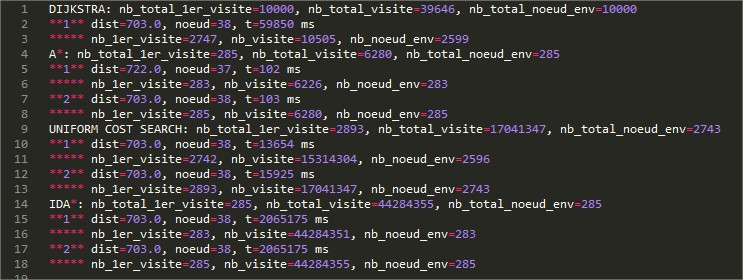
\includegraphics[width=1\textwidth]{./figures/log.jpg}
    \caption{Extrait du fichier de log du benchmarking sur 10 000 noeuds.}
\end{figure}

\clearpage

\chapter{Fichier d'une graine}

\begin{figure}[H]
\centering
    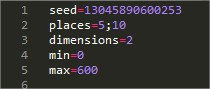
\includegraphics[width=0.5\textwidth]{./figures/seed.jpg}
    \caption{Extrait du fichier de la graine générant uen grille 2D de 5 sur 10 noeuds.}
\end{figure}

\clearpage

\section*{Résumé}
\addcontentsline{toc}{chapter}{Résumé}

\paragraph{Le sujet en bref.}
Le sujet qui a été choisi porte sur la réalisation d'un logiciel de benchmarking permettant de tester et de comparer différents algorithmes de recherche de plus court chemin sur des environnements générés par graine sur des séquences de tests. \newline

\paragraph{Les fonctionnalités implémentées.}

Génération et sauvegarde de grilles à N dimensions, benchmarkings de création d'environnement, visualisation graphique d'environnement 2D, création d'expérience de déploiement d'algorithmes sur les grilles, benchmarkings de déploiements d'algorithmes.

{\bf Mots-clés :} algorithmes de plus court chemin, théorie des graphes, environnements aléatoires, benchmarking, interface utilisateur, graines.

\end{document}